\section{Trainingsvorgang}

Der Trainingsvorgang basiert auf ein mehrschichtiges tiefes neuronales Netz, welches bereits im vorherigen Kapitel vorgestellt wurde. Dieses besteht aus folgenden Schichten:
\begin{description}
	\item Input-Schicht
	\item Hidden-Schicht 
	\item Output-Schicht
\end{description}
Bei den Eingangsdaten der Input-Schicht handelt es sich um beschriftete Sprachaufnahmen, die in die Netztopologie eingespeist werden. Eine Vorklassifizierung der Sprache führt zu einer erhöhten Spracherkennungsrate mehrerer Sprachen. Dies ging bereits aus {\cite{bishop.2006}} hervor. Das Training des Modells geschieht in der Hidden Layer-Schicht. Hier gilt es die Neuronen bzw. deren Gewichtungen entsprechend anzupassen. Im Kontext der Spracherkennung bedeutet dies, dass die Phoneme einer Sprachen extrahiert und erlernt werden müssen. Dabei wird die Sigmoidfunktion als Aktivitätsfunktion eingesetzt (s. Formel \ref{normal}). Diese Funktion beschreibt die Korrelation zwischen Input-Wert und  Aktivitätslevel eines Neurons. 
Der Input-Wert wird auf der X-Achse aufgetragen, das zugehörige Aktivitätslevel entsprechend auf die Y-Achse. Der Aktivitätslevel wird durch eine Ausgabefunktion in den Output transformiert, den das Neuron an andere Neuronen weitersendet\cite{Neuronal31:online}. Das Netz wird beginnend von der Input-Schicht bis zur Output-Schicht vollständig durchlaufen.  
\begin{equation}
sigm(x)=\frac{ 1 }{1+e^{-x}  }
\label{normal}
\end{equation}
Dabei wird eine Erweiterung des Backpropagation-Algorithmus eingesetzt. Die Backpropagation-Through-Time-Methode sorgt für das Berechnen der Gradienten. Diese werden im Gegensatz zum Standardalgorithmus über die einzelnen Zeitschritte aufsummiert. In dieser Erweiterung des Backpropagation, welche in Recurrent Neural Networks eingesetzt wird, werden lediglich die Parameter einzelnen Zeitschritte zwischen den Ebenen geteilt. Dieses Verfahren wird benötigt, um fehlerhafte Kantengewichte herauszufinden um diese anzupassen. Die Kantengewichte des Netzes werden mit null initialisiert. Die Ableitung der Sigmoid-Funktion wird bei der Korrekturberechnung notwendig (s. Formel \ref{ableitung}). Bei größeren Datenmengen entsteht ein Nachteil, welcher sich auf die Wissensausprägung des Netzes auswirkt. 
\\
Beim umgekehrten Durchlaufen entsteht allerdings ein Wissensverlust \cite{bishop.2006}. Dieser Verlust wird durch das Maxima der Ableitung $sigm(x)'$ repräsentiert. Dieser kann bis zu 25\% betragen. Der entstehende Verlust würde die Klassifizierungsrate des Trainingsmodels reduzieren, welches in Abbildung \ref{fig:features11.0} dargestellt ist \cite{Kulbear.2017}.
\begin{equation}
sigm(x)'= \frac{ e^{x} }{(e^{x} +1)^2  }
\label{ableitung}
\end{equation}

\begin{figure}[h!]
	\centering
	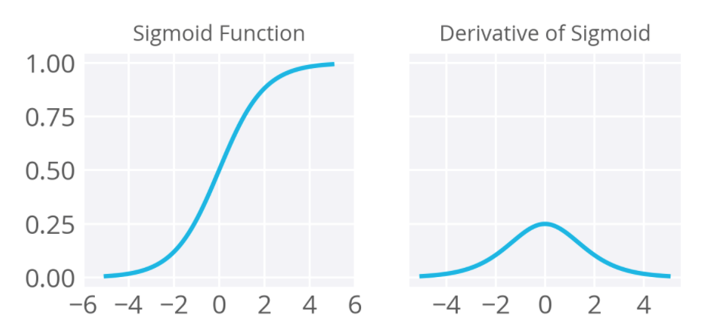
\includegraphics[width=1.0\linewidth]{images/sigmund}
	\caption{Darstellung der Sigmoid-Funktion und dessen Ableitung \cite{Kulbear.2017}} %Generelle
	\label{fig:features11.0}
\end{figure}
Anstelle der Sigmoid-Funktion wird in den heutigen Netzen jedoch die sogenannte Rectified Linear Units-Funktion ($ReLUs$) verwendet (s. Formel \ref{eq:ReLU}). Diese Funktion ist dem menschlichen Neuron am ähnlichsten und bringt zudem eine erhöhte Verarbeitungsgeschwindigkeit mit sich \cite{zeiler.2013}. Die Berechnung der Kantengewichte erfolgt durch Formel \ref{eq:Gewichte}).
\begin{equation}
y_{j} = ReLU(x_{j}) = max(0,x_{j}) 
\label{eq:ReLU}
%\caption{Rectiefied linear Units als Aktivierungsfunktion}
\end{equation}
\begin{equation}
x_{ j } = b_{ j } + \sum{ }{ }{ x_{ ij } * y_{j}}
\label{eq:Gewichte}
\end{equation}
Die Output-Schicht ordnet schließlich die Eingangsdaten den Klassen (Zielsprachen) zu. Diese Schicht ist als Softmax-Schicht konfiguriert, wie bereits aus dem letzten Kapitel hervorging. Die Klassen werden hier in einer eindimensionale Matrix kategorisiert. Dabei ist die Matrix in dem Zahlenintervall $[0,1]$ normalisiert. Die endgültige Sprachidentifikation geschieht über diese normalisierten Werte. Abbildung \ref{fig:soft} stellt dies dar. Die Werte lassen sich in Wahrscheinlichkeiten ausdrücken, indem sie mit dem Faktor 100 multipliziert werden \cite{Kulbear.2017}.
\begin{figure}[h!]
	\centering
	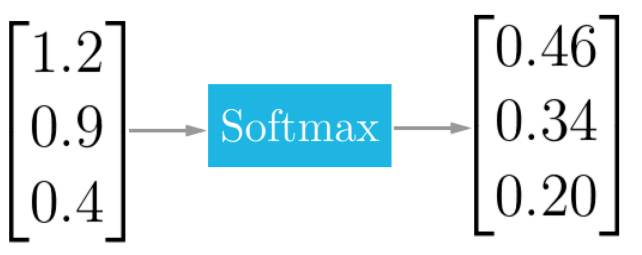
\includegraphics[width=0.7\linewidth]{images/softmax}
	\caption{Klassenzuordnung über Wahrscheinlichkeiten in der Softmax-Konfiguration \cite{Kulbear.2017}} %Generelle
	\label{fig:soft}
\end{figure}
 Die Vorhersagen der Output-Schicht geschieht durch die Funktion $p(j)$  (s. Formel \ref{eq:soft}). Dabei steht der Index l für die jeweilige Sprache.
\begin{equation}
p(j)= \frac{ exp(x_{j}) }{\sum_{l}{}{ exp(x_{l})} }
\label{eq:soft}
\end{equation}
Für das vorhin erwähnte Backpropagation-Verfahren wird ebenfalls eine Kostenfunktion benötigt. Diese geschieht durch die Cross-Entropy-Loss-Funktion. Diese Funktion misst die Abweichungen der Kantengewichte der Netztopologie und passt diese rückwirkend an. Der Cross-Entropy-Verlust nimmt zu, wenn der vorhergesagte Wert von der tatsächlichen Beschriftung abweicht \cite{MLCheatsheet.2017}. Bei $t_{j}$ handelt es sich um die Klasse, für die der Verlust berechnet wird \cite{GonzalezDominguez.2015}.
\begin{equation}
C= \sum_{l}{}{ t_{j} * log(p_{j})} 
\label{eq:back}
\end{equation}

\subsection{Netztopologie}
Die Netztopologie beschreibt die Infrastruktur des Netzes. Die Auswahl der Topologie bestimmt die Qualität des Trainingsvorgangs. Eine zu geringe Anzahl der Neuronen führt zu einer niedrigen Spracherkennungsrate. Eine zu hohe Anzahl würde zu einer überhöhten Trainingsdauer führen. Die Topologien unterscheiden sich zwischen verschiedenen Ansätzen und liefern Spracherkennungsresultate \cite{bishop.2006}. 

In dieser Arbeit wird der Topologienvorschlag von Gonzales et al. betrachtet. Für die Eingangsdaten werden 40 Filterbanken verwendet. In der Input-Schicht werden 26 Neuronen eingesetzt. Um unerwünschte Latenzzeiten zu vermeiden, wird ein asymmetrischer Kontext verwendet. Die Hidden-Schicht beträgt vier Ebenen mit einer Gesamtzahl von 2560 Neuronen. Die Output-Schicht enthält die Softmax-Konfiguration. Dies ist bei der Erkennung von multilingualen Sprachen eine erforderliche Konfiguration \cite{GonzalezDominguez.2015}.
 
%\begin{figure*}[h!]
%	\centering
%	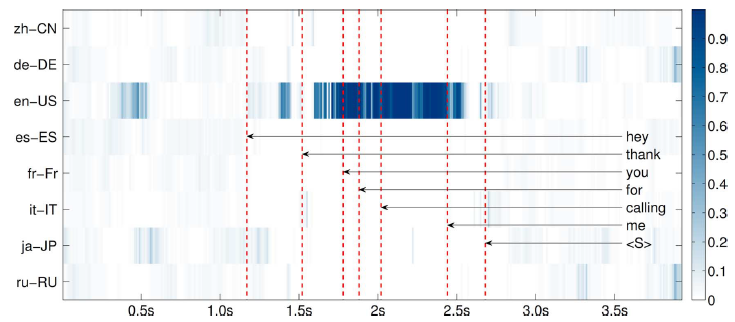
\includegraphics[width=1.0\linewidth]{images/Output}
%	\caption{Netztopologie zur  \cite{GonzalezDominguez.2015}} %Generelle
%	\label{fig:topology}
%\end{figure*}
\subsection{Verbesserung des Trainingsverfahrens durch Multitasking learning (MTL)}
 Bei maschinellem Lernen wird der Fokus auf das Optimieren bestimmte Metriken gesetzt. Dazu zählen beispielsweise die Klassifizierungsgenauigkeit und Trainingsdauer. Das Lernen der einzelnen Sprachen läuft sequenziell ab. Hier wird das Multitasking Learning (MTL) eingesetzt. Dieser Ansatz zielt darauf ab, die Generalisierungsleistung einer Lernaufgabe zu verbessern. Dies wird erreicht, indem mehrere zusammenhängende Aufgaben gemeinsam gelernt werden und nicht sequentiell. Dies bedeutet jedoch nicht, dass die Aufgaben ähnlich sind. Sie müssen lediglich auf verschiedene Ebenen abstrahiert und geteilt werden. Dabei lässt sich das Wissen zwischen Aufgaben übertragen. Es wurde festgestellt, dass gemeinsames Lernen dafür sorgt, dass Wissen miteinander ausgetauscht wird und somit die Trainingsdauer verkürzt. Folglich hilft eine so gewonnene interne Repräsentation den Modellen, zukünftige Daten besser zu verallgemeinern. Beim gemeinsamen Nutzen der Phoneme findet dieser Ansatz somit Verwendung {\cite{multitask}}. MLT ist auch nützlich, wenn die Menge der markierten Daten im Vergleich zur Modellgröße gering ausfällt. Das bedeutet, dass das geteilte Wissen der Ressourcenknappheit einiger Sprachen zugute kommt. Dieser Mangel an Sprachressourcen ist ein Hindernis automatischer Spracherkennungssysteme. Es werden grundsätzlich zwei Arten von MTL unterschieden: Hard- und Soft Parameter Sharing.\newline\newline
 Hard Parameter Sharing stellt die meist genutzte Art dar\cite{Ruder.2017}. Es wird auf die Hidden-Schicht angewendet, indem sich die Aufgaben gemeinsam lernen lassen, während die spezifischen Aufgaben separat erlernt werden. Dies wird in Abbildung \ref{fig:hard} dargestellt. Der Ansatz reduziert das Overfitting-Risiko. Je mehr Aufgaben gleichzeitig erlernt werden, desto mehr muss das Modell eine Repräsentation finden, die sämtliche Aufgaben erfassen muss. Somit ist die Chance auf Overfitting geringer \cite{Ruder.2017} \cite{Lu_multitasklearning}.
  \begin{figure}[h!]
 	\centering
 	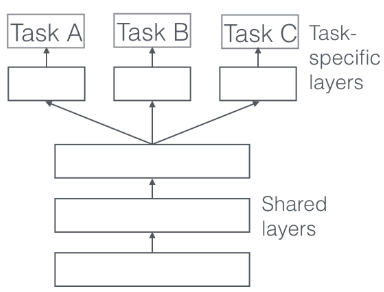
\includegraphics[width=0.8\linewidth]{images/hard}
 	\caption{Hard parameter sharing auf die Hidden-Schicht angewendet \cite{Kulbear.2017}.} %Generelle
 	\label{fig:hard}
 \end{figure}

